\begin{sectionbox}{La electricidad en el cuerpo humano}
    Las neuronas se comunican entre sí mediante señales eléctricas que recorren el axón
    de la neurona y se propagan a otras neuronas mediante la sinapsis, que es la zona
    donde se conecta una neurona con otra (figura \ref{fig:20230502024056}a).
    La figura \ref{fig:20230502024056}b representa la membrana de una célula nerviosa que no interactúa
    con ninguna otra neurona (en estas condiciones se dice que la neurona se encuentra
    en reposo).
    \begin{figure}[H]
        \centering
        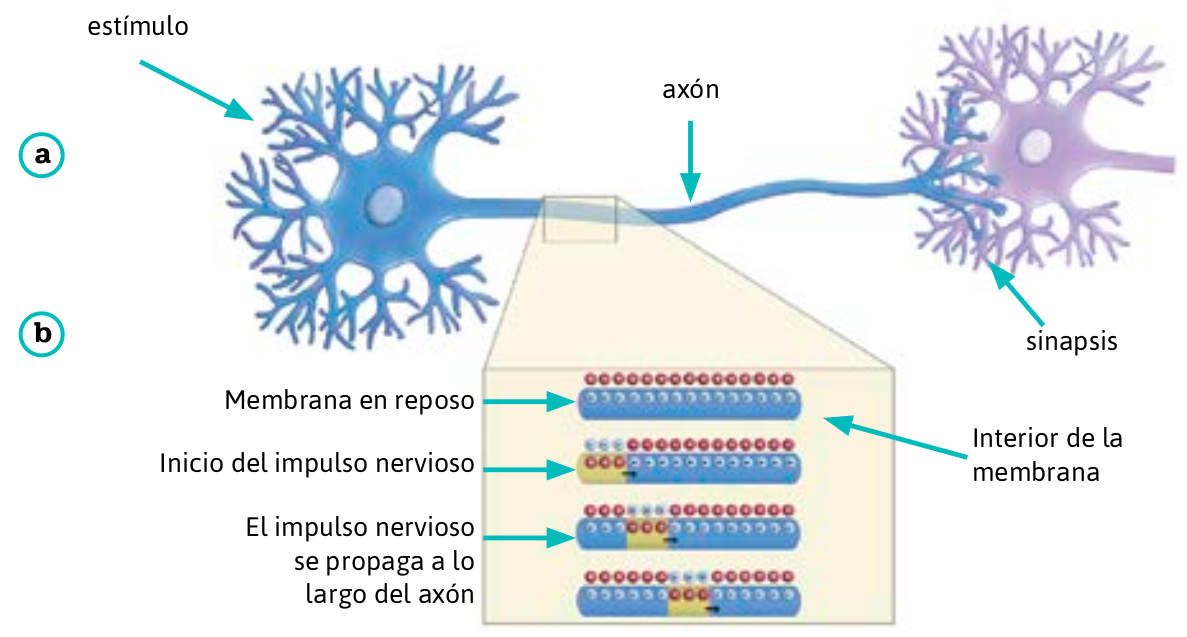
\includegraphics[width=0.8\linewidth]{../images/20230502024056}
        \caption{El pulso eléctrico que se propaga a través de la neurona también se conoce como potencial de acción.}
        \label{fig:20230502024056}
    \end{figure}

    \begin{minipage}{0.55\textwidth}
        Observa que el exterior de membrana tiene carga positiva y que el interior
        está cargado negativamente. Cuando una neurona recibe un estímulo, las cargas eléctricas en el exterior y el interior de la membrana se invierten en el punto de la estimulación, lo cual genera una perturbación eléctrica, llamada impulso nervioso, que
        se propaga a través de la membrana. La frecuencia de estas ondas, así como su forma
        y otras características constituyen el \comillas{lenguaje} por medio del cual las neuronas se
        comunican entre sí. ¿Cuál es el origen de la electricidad con la que se comunican las neuronas? ¿De
        dónde proviene la carga eléctrica?

        Galvani pensaba que la \comillas{electricidad animal} era
        un fluido que se generaba en el interior de los organismo y que viajaba por la sangre
        y los nervios, pero el físico italiano Alessandro Volta no estaba de acuerdo con él.
        Volta sostenía que las contracciones de las ancas de rana en el experimento de Galvani
        no se debían a que sus músculos tuvieran cierta cantidad de electricidad, sino al contacto entre el zinc y el cobre, y que las patas de la rana sólo reaccionaban a esa electricidad; sin embargo, en aquella época no había instrumentos que permitieran demostrar
        si en la propia pata se generaba corriente.

        No fue hasta 1952 cuando los biofísicos \textbf{Alan
        Hodgkin (1914-1998)} y \textbf{Andrew Huxley (1917-2012)}
        (medio hermano del novelista Aldous Huxley) demostraron que la electricidad de los organismos funciona mediante iones, los cuales
        son átomos a los que les faltan o sobran electrones, es
        decir, están eléctricamente cargados.

    \end{minipage}\hfill
    \begin{minipage}{0.42\textwidth}
        \begin{figure}[H]
            \centering
            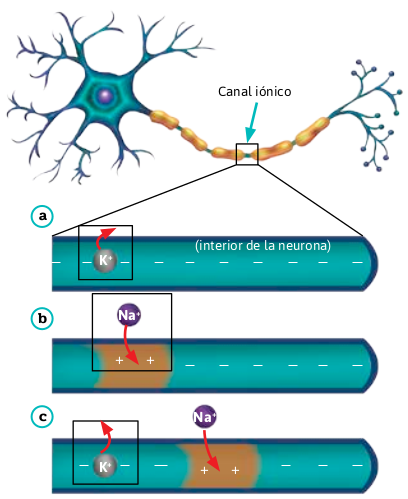
\includegraphics[width=0.95\linewidth]{../images/20230502034142}
            \caption{La membrana de las células nerviosas permite el
                paso de iones positivos al interior y exterior de las neuronas,
                generalmente sodio (Na$^+$) y potasio (K$^+$).}
            \label{fig:20230502034142}
        \end{figure}
    \end{minipage}

    Según el planteamiento de Hodgkin y Huxley, la membrana de las neuronas poseen estructuras, llamadas
    canales iónicos, que permiten el paso de iones a través de la membrana. Cuando la neurona se encuentra en
    estado de reposo, los canales iónicos sólo permiten el
    paso de iones positivos al exterior (figura \ref{fig:20230502034142}a). Si la
    neurona recibe un estímulo, los canales iónicos también
    admiten el paso de iones positivos al interior de la neurona, lo que altera la carga eléctrica de la membrana
    en el punto de la estimulación (figura \ref{fig:20230502034142}b) y permite
    (interior de la neurona) la propagación del estímulo a la zona contigua.
    Un instante después (del orden de milisegundos) otro canal iónico libera iones positivos al exterior para restaurar
    el signo de la carga eléctrica al estado de reposo (figura \ref{fig:20230502034142}c). De esta manera se propaga la señal nerviosa.

    \begin{minipage}{0.55\textwidth}
        \begin{figure}[H]
            \centering
            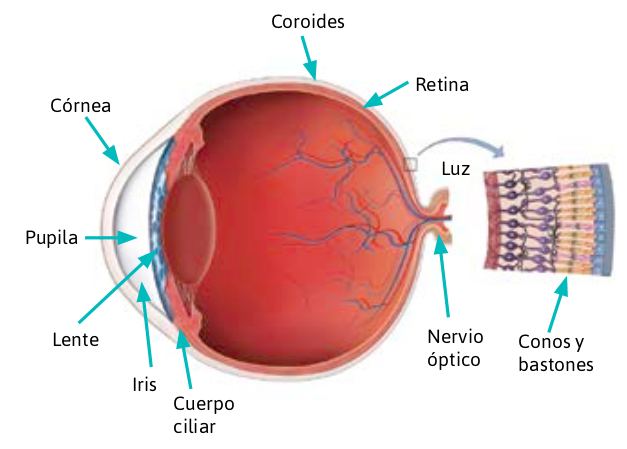
\includegraphics[width=0.9\linewidth]{../images/20230502025101}
            \caption{En la retina de nuestros ojos tenemos dos tipos de células que contraerse o relajarse. }
            \label{fig:20230502025101}
        \end{figure}
    \end{minipage}\hfill
    \begin{minipage}{0.4\textwidth}
        Las neuronas no son las únicas células de nuestro cuerpo en las que intervienen fenómenos eléctricos.
        Las células de nuestros ojos, las de nuestros músculos y también las de nuestro corazón emplean electricidad.
        En nuestros ojos tenemos dos tipos de células que reaccionan ante la luz y los colores: los conos y los bastones. Estas células poseen un tipo especial de
        Estas células poseen un tipo especial de canales iónicos que se activan con la luz. Los bastones se activan
        en la oscuridad o con poca luz y perciben las intensidades luminosas entre el negro y el blanco, pasando por todas las tonalidades de gris. Los conos son células receptoras capaces de percibir
        colores, pero para que funcionen es necesario que haya suficiente
        luz. ¿Has notado que en una noche oscura o muy temprano no
        se pueden ver los colores? Existen tres tipos de conos, cada uno capaz de percibir uno de los tres colores primarios
        (rojo, verde o azul), que combinados dan todos los colores del espectro visible, de modo que no necesitamos más.
    \end{minipage}

    Cada célula de nuestra retina estimula al nervio óptico para enviar señales eléctricas al cerebro, que las interpreta como luz, color e imágenes.
    ¿Entonces, tal vez puedas imaginarte, con qué vemos, con nuestros ojos o con nuestro cerebro?
    En los músculos y el corazón la electricidad produce movimiento; el cerebro envía señales a las células de los músculos y del corazón para activar sus canales iónicos y que éstos puedan contraerse o relajarse (ver figura \ref{fig:20230502025101}).
\end{sectionbox}